\hypertarget{intro}{%
\chapter{Introduction}\label{intro}}

In this class, we will use the R language, and the RStudio integrated development environment (IDE). Before the first meeting, install the necessary software on your personal computer by executing the following instructions.

\hypertarget{installing-r-and-rstudio}{%
\section{Installing R and Rstudio}\label{installing-r-and-rstudio}}

Go to the website of the Comprehensive R Archive Network (\url{https://cran.r-project.org/}) and download the latest version of R for your operating system (Windows, MacOS, or Linux). As of \today, the latest version is 4.0.4. Follow the installation instructions.

Next, go the Rstudio download website
(\url{https://rstudio.com/products/rstudio/download/}) and get the Desktop version
(open source license). As of \today, the version is 1.4.1106. Follow the
installation instruction. An icon that looks like this:

\includegraphics[width=\textwidth,height=0.025\textheight]{images/RstudioLogo.png}
will be on your computer's desktop. Double-click on this icon to start the R session. The Rstudio IDE will open, and look like this:

\begin{center}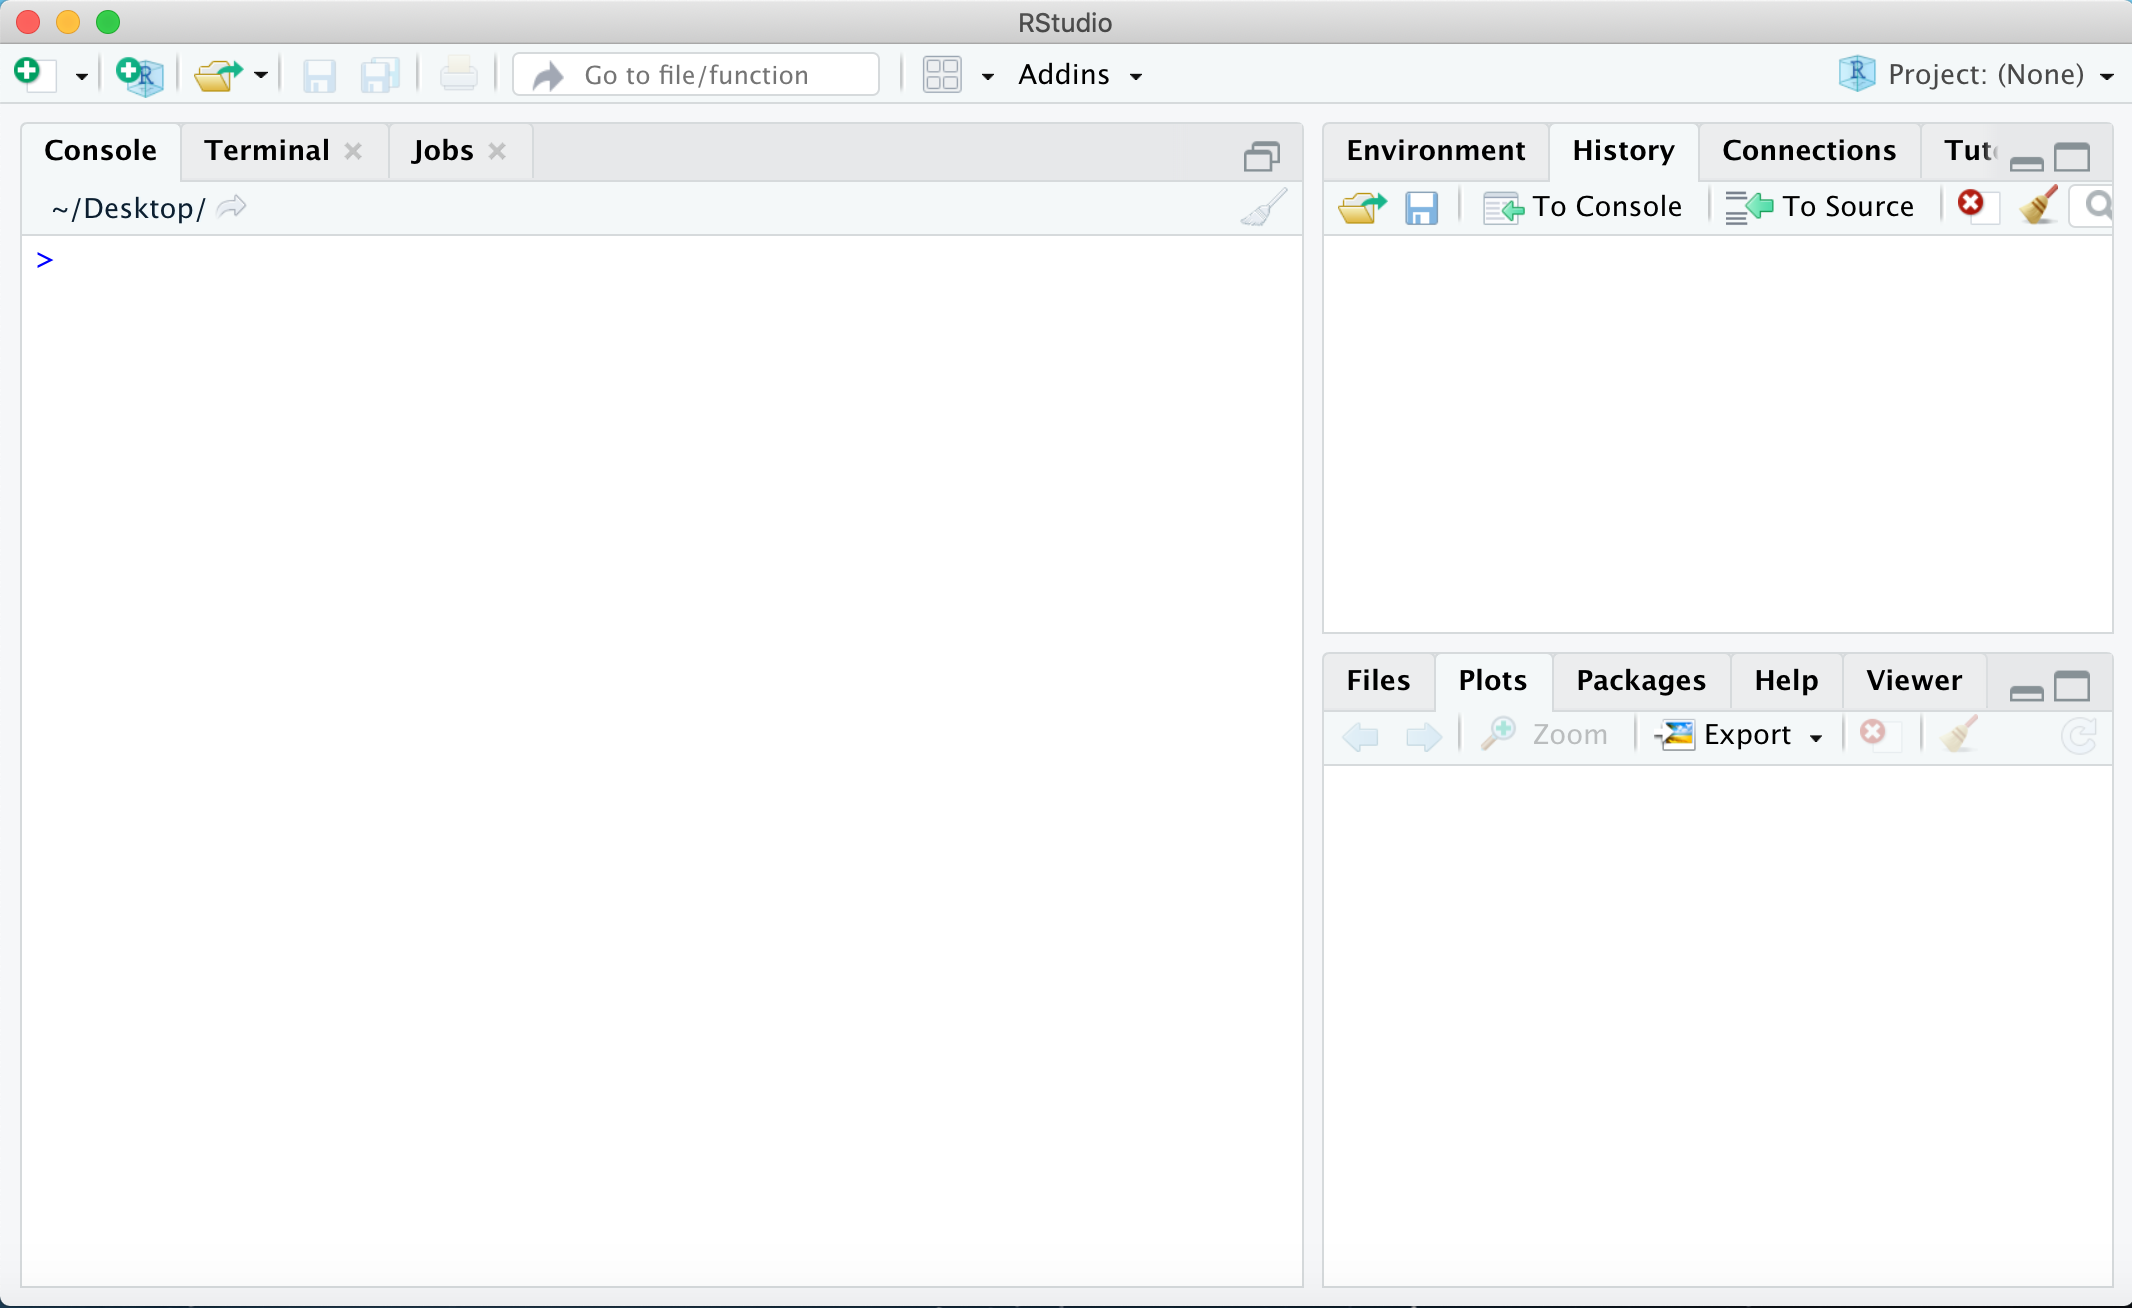
\includegraphics[width=0.7\linewidth]{images/RstudioMain} \end{center}

The left-hand side of the screen contains the Console tab. Notice the \(>\) sign (called the `prompt'). When you see this character, it means the R is ready for the next command. Put the cursor there, and then type

\begin{verbatim}
2 + 2
\end{verbatim}

and hit Enter on the keyboard. You should get the following on the Console:

\begin{verbatim}
[1] 4
\end{verbatim}

Notice the top-right part of the Rstudio window. You should see an `Environment' and a `History' tab. Click on History. Notice that your previous input appears there. Try entering another calculation or command and see that they appear in the session's history. For example, try entering the following

\begin{Shaded}
\begin{Highlighting}[]
\DecValTok{3} \SpecialCharTok{\^{}} \DecValTok{5}
\FunctionTok{date}\NormalTok{()}
\end{Highlighting}
\end{Shaded}

Click on the Environment tab. It should be empty when you start R for the first time. In the Console, type

\begin{Shaded}
\begin{Highlighting}[]
\NormalTok{myFirstVariable }\OtherTok{\textless{}{-}} \FunctionTok{factorial}\NormalTok{(}\DecValTok{5}\NormalTok{)}
\end{Highlighting}
\end{Shaded}

Notice that nothing was printed in the Console, but the Environment tab now contains a table with one row, with `myFirstVariable' appearing in the cell on the left, and its value (120) on the right. Any object appearing in the Environment tab is available to you throughout your R session, and you don't have to recalculate it. For example, you can try the following:

\begin{Shaded}
\begin{Highlighting}[]
\NormalTok{myFirstVariable}\SpecialCharTok{/}\DecValTok{6}
\end{Highlighting}
\end{Shaded}

The Console should now display 20.

The lower-right side of the IDE contains a file browser (the Files tab), information about installed packages (more about it later), and any plot generated during the R session. It also contains a Help tab, to obtain information about built-in functions.

Finally, before we move on to the next section, in the Rstudio top menu, click on File, then on New File, and then on R Script. Alternatively, you can click on little green `+' icon in the top-left part of the IDE. This will split the left side of the Rstudio IDE into two parts -- the lower part will contain the Console, and the top part will contain a tab labeled `Untitled1'. This is were you can enter R code which you will save to a permanent file, and re-use later.
For example, enter the following in the blank space in the Untitled1 tab:

\begin{Shaded}
\begin{Highlighting}[]
\CommentTok{\# This is my first R program}
\FunctionTok{cat}\NormalTok{(}\StringTok{\textquotesingle{}Hello, World!}\SpecialCharTok{\textbackslash{}n}\StringTok{\textquotesingle{}}\NormalTok{)}
\end{Highlighting}
\end{Shaded}

Then, click on File \(>\) Save, and in the `Save As' box enter FirstProgram.R and click the Save button.
Notice that the tab name is now FirstProgram.R.

In that part of the window, there should now be a small button called Source. Click on it. The program will be executed and the output will be shown in the Console. You can also execute individual lines in the source code. Just put the cursor anywhere in that line, and click on the Run button (which is near the Source button.)

That's it. In the rest of these notes we will see more features of Rstudio, but you are now ready to start learning programming in R.
